
%butter
\textbf{Butterworth}
\begin{itemize}
    \item center frequency $f_c$
    \begin{itemize}
        \item center frequency $f_c$ is given by ${f_c}^2={f_{c1}}^2*{f_{c2}}^2$
		\item zero phaseshift @center frequency $f_c$
    \end{itemize}
    \item @lower cut-off frequency~ $f_{c1}$
    \begin{itemize}
        \item -3dB attenuation
        \item 45 degree phaseshift
    \end{itemize}
	\item @upper cut-off frequency~$f_{c2}$
    \begin{itemize}
        \item -3dB attenuation
        \item -45 degree phaseshift
    \end{itemize}
    \item stopband 
    \begin{itemize}
        \item monotonic -20dB decline per decade
		\item roll-off dynamics are constant and not adjustable
    \end{itemize} 
\end{itemize}

E.g.: \\
The cut-off frequencies are $f_{c1}=10$Hz and $f_{c2}=100$Hz.\\
The bodeplot is shown in the figure \ref{fig:bp_butter} below.
\begin{figure}[h!]
  \centering
  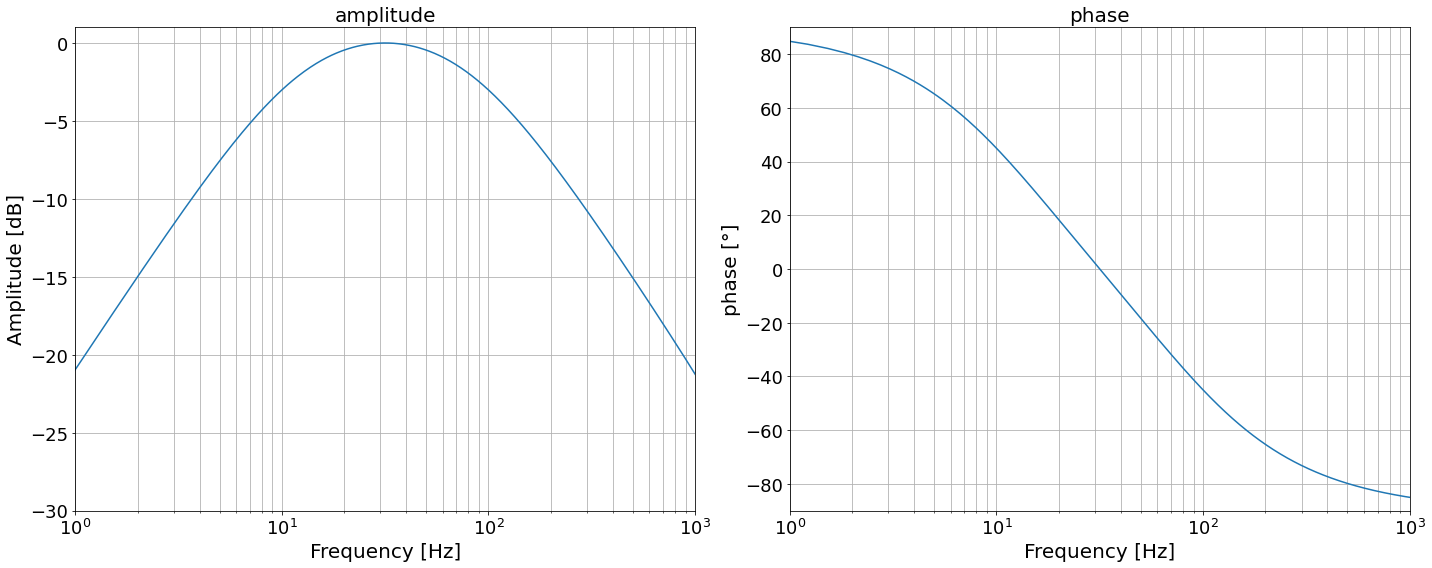
\includegraphics[width=.75\linewidth]{bp_butter.png}
  \caption{Bodeplot Butterworth bandpass.}
  \label{fig:bp_butter}
\end{figure}
	
% Cheby
\textbf{Chebyshev}\\
\emph{Note:} A second order Chebyshev I bandpass has the same bodeplot as a second order Chebyshev II bandpass. Hence, only the 'Chebyshev' option is given.\\
\begin{itemize}
    \item center frequency $f_c$
    \begin{itemize}
        \item center frequency $f_c$ is given by ${f_c}^2={f_{c1}}^2*{f_{c2}}^2$
		\item zero phaseshift @center frequency $f_c$
    \end{itemize}
    \item @lower cut-off frequency~ $f_{c1}$
    \begin{itemize}
        \item $-rc$dB attenuation
        \item phaseshift proportional to $rc$
    \end{itemize}
	\item @upper cut-off frequency~$f_{c2}$
    \begin{itemize}
        \item $-rc$dB attenuation
        \item -phaseshift proportional to $rc$
    \end{itemize}
    \item stopband 
    \begin{itemize}
        \item monotonic -20dB decline per decade
		\item roll-off dynamics are adjustable using parameter $rc$
    \end{itemize} 
\end{itemize}


E.g.: \\
The cut-off frequencies are $f_{c1}=10$Hz and $f_{c2}=100$Hz.\\
The parameter $rc$ is set to $10$dB.\\
The bodeplot is shown in the figure \ref{fig:bp_cheby1} below.
\begin{figure}[h!]
  \centering
  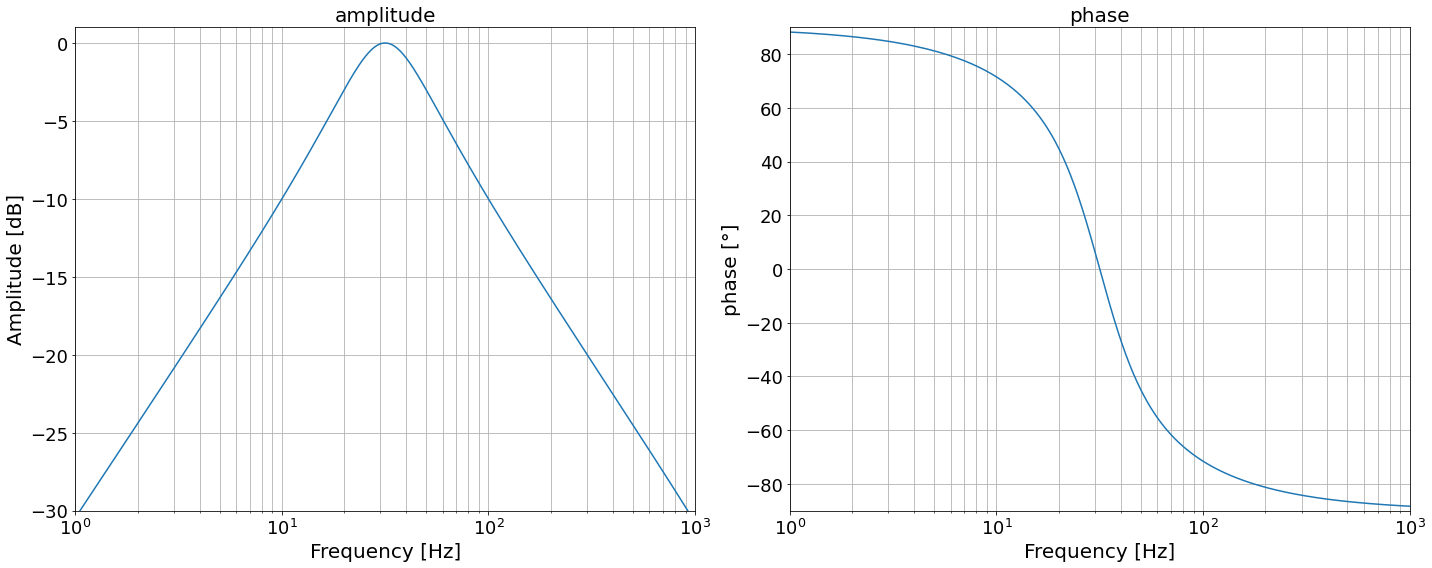
\includegraphics[width=.75\linewidth]{bp_cheby1.png}
  \caption{Bodeplot Chebyshev bandpass. $rc=10$dB}
  \label{fig:bp_cheby1}
\end{figure}

%bessel
\textbf{Bessel}\\
\emph{Note:} A second order Bessel bandpass behaves exactly like a second order Butterworth bandpass. Hence, no 'Bessel' option is given.